%\chapter{\normalsize{BACKGROUND OF SATELLITE REMOTE SENSING}}
\chapter{\normalsize{CASE STUDY: GOES-R Series}}
\section{GOES project current status}
\paragraph{}
The Geostationary Operational Environmental Satellite Program (GOES) is a joint effort of NASA and the National Oceanic and Atmospheric Administration (NOAA). The GOES system currently consists of GOES-13, operating as GOES-East, in the eastern part of the constellation at 75 degrees west longitude and GOES-15, operating as GOES-West, at 135 degrees west longitude. The GOES-R series will maintain the two-satellite system implemented by the current GOES series. However, the locations of the operational GOES-R satellites will be 75 degrees west longitude and 137 degrees west longitude. The latter is a shift in order to eliminate conflicts with other satellite systems. The GOES-R series operational lifetime extends through December 2036.
These spacecraft help meteorologists observe and predict local weather events, including thunderstorms, tornadoes, fog, hurricanes, flash floods and other severe weather. In addition, GOES observations have proven helpful in monitoring dust storms, volcanic eruptions and forest fires.The benefits that directly enhance the quality of human life and protection of Earth's environment include:
\begin{itemize} 
\item Supporting the search-and-rescue satellite aided system (SARSAT).
\item Contributing to the development of worldwide environmental warning services and enhancements of basic environmental services.
\item Improving the capability for forecasting and providing real-time warning of solar disturbances.
\item Providing data that may be used to extend knowledge and understanding of the atmosphere and its processes.
\end{itemize}	
The next series of GOES satellites includes GOES-R, S, T and U.
\newpage
\section{GOES-R Series Instruments}
\paragraph{}
GOES-R Series has six instruments on board:
\begin{description}
\item[Earth-pointing] : 
\begin{itemize} 
\item Advanced Baseline Imager (ABI) - the primary instrument for imaging Earth’s weather, oceans and environment.
\item Geostationary Lightning Mapper (GLM) - a single-channel, near-infrared optical transient detector that can identify momentary changes in an optical scene, indicating the presence of lightning.
\end{itemize}
\item[Sun-pointing] : 
\begin{itemize} 
\item Extreme Ultraviolet and X-ray Irradiance Sensors (EXIS) - monitors solar irradiance in the upper atmosphere using two primary sensors: the Extreme Ultraviolet Sensor (EUVS) and the X-Ray Sensor (XRS).
\item  Solar Ultraviolet Imager (SUVI) - a telescope that monitors the sun in the extreme ultraviolet wavelength range, detecting solar flares and solar eruptions, and compiling full disk solar images.
\end{itemize}
\item[In-situ] : 
\begin{itemize} 
\item Magnetometer (MAG) - measures the space environment magnetic field that controls charged particle dynamics in the outer region of the magnetosphere
\item Space Environment In-Situ Suite (SEISS) - monitors proton, electron, and heavy ion fluxes in the magnetosphere using four sensors: the Energetic Heavy Ion Sensor (EHIS), the High and Low Magnetospheric Particle Sensors (MPS-HI and MPS-LO), and the Solar and Galactic Proton Sensor (SGPS).
\end{itemize}
\end{description}
Only two sensors are used for atmospheric purpose, Advanced Baseline Imager (ABI) and Geostationary Lightning Mapper (GLM).
\newpage
\section{Advanced Baseline Imager (ABI)}
ABI is a multi-channel passive imaging radiometer that images Earth’s weather, oceans and environment with 16 spectral bands (2 visible, 4 near-infrared, and 10 infrared channels).

\begin{figure}[H]
\begin{center}
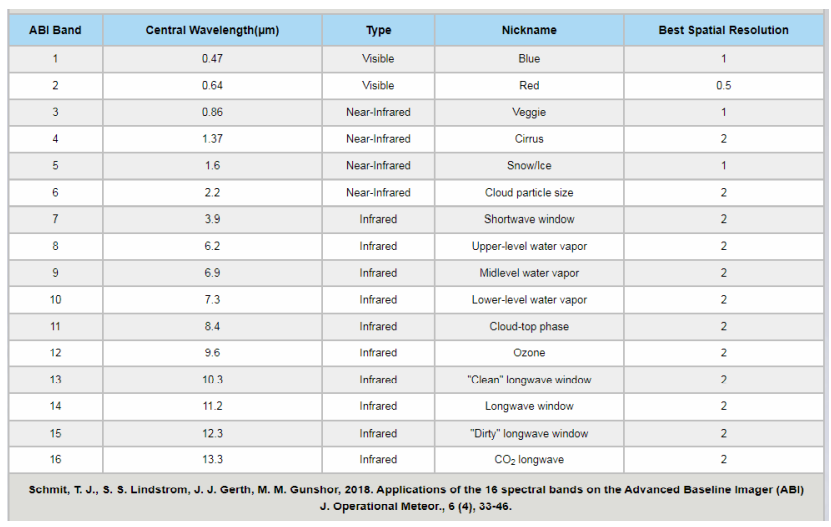
\includegraphics[scale=0.8]{abi_band_image.png} %\cite{umhe}
\end{center}
\caption{ABI optical components}
\label{ABI optical components}%\cite{ABIA}
\end{figure}
\section{ABI modes of operation}
\paragraph{}
ABI has four modes of operation.
\begin{description}
\item[Full Disk] : Hemispheric Coverage of 83° local zenith angle, temporal resolution of 5-15 minutes, and spatial resolution of 0.5 to 2km.
\item[ Mesoscale]: Provides coverage over a 1000x1000km box with a temporal resolution of 30 seconds, and spatial resolution of 0.5 to 2km.
\item[ Continental US/Pacific US]: The CONUS and PACUS scans are performed every five minutes, providing coverage of the 5000km (east/west) and 3000km (north/south) rectangle over the continental United States (GOES-16) or the Pacific Ocean, including Hawaii (GOES-17). The spatial resolution is 0.5 to 2km.
\item[ Flex Modes]: The flex modes provide a full disk scan every 10 minutes (mode 6) or every 15 minutes (mode 3), a CONUS/PACUS every five minutes, and two mesoscale domains every 60 seconds (or one sub-region every 30 seconds).
\end{description}

\section{GOES-R Data Products}
\paragraph{}
GOES-R Data products have three levels.
\begin{description}
\item [Level 0 (L0)] : are observation data received directly from the 6 satellite instruments. The data is not meaningful to most users prior to processing by the ground system.
\item [Level 1b (L1b)] : are calibrated and, where applicable, geographically corrected, L0 data. This means that the data has been processed so that its values are in standard units of physical quantities. For ABI, the L1b product is Radiances.
This is useful for users who require radiance units, instead of reflectance/brightness temperature (Kelvin) units.
All of the instruments have L1b products available except GLM, which is only distributed as an L2+ product.
\item [Level 2+ Products] : contain environmental physical qualities, such as cloud top height or land surface temperature.
Aside from the GLM Lightning Detection Product, the data source for these products is the ABI L1b data.
\end{description}
\section{ABI meteorological product}
\paragraph{}
The mission-critical ABI product is \href{https://www.goes-r.gov/products/baseline-cloud-moisture-imagery.html}{Cloud and Moisture Imagery} (CMI), which utilizes all 16 ABI spectral bands,
and is used to generate an array of products aiding forecasters in monitoring and predicting weather hazards.
The following is a list ABI meteorological and space weather data products that are available to the user community.
\begin{itemize} 
\item \href{https://www.goes-r.gov/products/baseline-aerosol-detection.html}{Aerosol detection (including smoke and dust)} 
\item \href{https://www.goes-r.gov/products/baseline-aerosol-opt-depth.html}{Aerosol optical depth (AOD)}
\item \href{https://www.goes-r.gov/products/opt2-aerosol-particle-size.html}{Aerosol particle size}
\item \href{https://www.goes-r.gov/products/baseline-clear-sky-mask.html}{Clear sky masks}
\item \href{https://www.goes-r.gov/products/opt2-cloud-layers-height.html}{Cloud layers/heights}
\item \href{https://www.goes-r.gov/products/baseline-cloud-moisture-imagery.html}{Cloud and moisture imagery}
\item \href{https://www.goes-r.gov/products/baseline-cloud-opt-depth.html}{Cloud optical depth}
\item \href{https://www.goes-r.gov/products/baseline-cloud-particle-size-dist.html}{Cloud particle size distribution}
\item \href{https://www.goes-r.gov/products/baseline-cloud-top-height-cloud-layer.html}{Cloud top height} 
\item \href{https://www.goes-r.gov/products/baseline-cloud-phase.html}{Cloud top phase}
\item \href{https://www.goes-r.gov/products/baseline-cloud-top-pressure.html}{Cloud top pressure}
\item \href{https://www.goes-r.gov/products/baseline-cloud-top-temp.html}{Cloud top temperature}
\item \href{https://www.goes-r.gov/products/baseline-derived-motion-winds.html}{Derived motion winds}
\item \href{https://www.goes-r.gov/products/baseline-derived-stability-indices.html}{Derived stability indices}
\item \href{https://www.goes-r.gov/products/baseline-DSR.html}{Downward shortwave radiation: surface}
\item \href{https://www.goes-r.gov/products/baseline-fire-hot-spot.html}{Fire/hot spot characterization}
\item \href{https://www.goes-r.gov/products/baseline-hurricane-intensity.html}{Hurricane intensity estimation}
\item \href{https://www.goes-r.gov/products/LSA.html}{Land surface albedo}
\item \href{https://www.goes-r.gov/products/BRF.html}{Land surface bidirectional reflectance factor}
\item \href{https://www.goes-r.gov/products/baseline-LST.html}{Land surface temperature (skin)}
\item \href{https://www.goes-r.gov/products/baseline-legacy-vert-moisture-profile.html}{Legacy vertical moisture profile}
\item \href{https://www.goes-r.gov/products/baseline-legacy-vert-temp-profile.html}{Legacy vertical temperature profile}
\item \href{https://www.goes-r.gov/products/baseline-radiances.html}{Radiances}
\item \href{https://www.goes-r.gov/products/baseline-rainfall-rate-qpe.html}{Rainfall rate/QPE}
\item \href{https://www.goes-r.gov/products/baseline-TOA.html}{Reflected shortwave radiation: TOA}
\item \href{https://www.goes-r.gov/products/opt2-sea-lake-ice-age.html}{Sea and lake ice: age}
\item \href{https://www.goes-r.gov/products/opt2-sea-lake-ice-concentration.html}{Sea and lake ice: concentration}
\item \href{https://www.goes-r.gov/products/opt2-sea-lake-ice-motion.html}{Sea and lake ice: motion}
\item \href{https://www.goes-r.gov/products/baseline-SST.html}{Sea surface temperature (skin)}
\item \href{https://www.goes-r.gov/products/baseline-snow-cover.html}{Snow cover}
\item \href{https://www.goes-r.gov/products/baseline-total-precipitable-water.html}{Total precipitable water}
\item \href{https://www.goes-r.gov/products/baseline-volcanic-ash.html}{Volcanic ash: detection and height}
\end{itemize}


